
% Default to the notebook output style

    


% Inherit from the specified cell style.




    
\documentclass[11pt]{article}

    
    
    \usepackage[T1]{fontenc}
    % Nicer default font (+ math font) than Computer Modern for most use cases
    \usepackage{mathpazo}

    % Basic figure setup, for now with no caption control since it's done
    % automatically by Pandoc (which extracts ![](path) syntax from Markdown).
    \usepackage{graphicx}
    % We will generate all images so they have a width \maxwidth. This means
    % that they will get their normal width if they fit onto the page, but
    % are scaled down if they would overflow the margins.
    \makeatletter
    \def\maxwidth{\ifdim\Gin@nat@width>\linewidth\linewidth
    \else\Gin@nat@width\fi}
    \makeatother
    \let\Oldincludegraphics\includegraphics
    % Set max figure width to be 80% of text width, for now hardcoded.
    \renewcommand{\includegraphics}[1]{\Oldincludegraphics[width=.8\maxwidth]{#1}}
    % Ensure that by default, figures have no caption (until we provide a
    % proper Figure object with a Caption API and a way to capture that
    % in the conversion process - todo).
    \usepackage{caption}
    \DeclareCaptionLabelFormat{nolabel}{}
    \captionsetup{labelformat=nolabel}

    \usepackage{adjustbox} % Used to constrain images to a maximum size 
    \usepackage{xcolor} % Allow colors to be defined
    \usepackage{enumerate} % Needed for markdown enumerations to work
    \usepackage{geometry} % Used to adjust the document margins
    \usepackage{amsmath} % Equations
    \usepackage{amssymb} % Equations
    \usepackage{textcomp} % defines textquotesingle
    % Hack from http://tex.stackexchange.com/a/47451/13684:
    \AtBeginDocument{%
        \def\PYZsq{\textquotesingle}% Upright quotes in Pygmentized code
    }
    \usepackage{upquote} % Upright quotes for verbatim code
    \usepackage{eurosym} % defines \euro
    \usepackage[mathletters]{ucs} % Extended unicode (utf-8) support
    \usepackage[utf8x]{inputenc} % Allow utf-8 characters in the tex document
    \usepackage{fancyvrb} % verbatim replacement that allows latex
    \usepackage{grffile} % extends the file name processing of package graphics 
                         % to support a larger range 
    % The hyperref package gives us a pdf with properly built
    % internal navigation ('pdf bookmarks' for the table of contents,
    % internal cross-reference links, web links for URLs, etc.)
    \usepackage{hyperref}
    \usepackage{longtable} % longtable support required by pandoc >1.10
    \usepackage{booktabs}  % table support for pandoc > 1.12.2
    \usepackage[inline]{enumitem} % IRkernel/repr support (it uses the enumerate* environment)
    \usepackage[normalem]{ulem} % ulem is needed to support strikethroughs (\sout)
                                % normalem makes italics be italics, not underlines
    

    
    
    % Colors for the hyperref package
    \definecolor{urlcolor}{rgb}{0,.145,.698}
    \definecolor{linkcolor}{rgb}{.71,0.21,0.01}
    \definecolor{citecolor}{rgb}{.12,.54,.11}

    % ANSI colors
    \definecolor{ansi-black}{HTML}{3E424D}
    \definecolor{ansi-black-intense}{HTML}{282C36}
    \definecolor{ansi-red}{HTML}{E75C58}
    \definecolor{ansi-red-intense}{HTML}{B22B31}
    \definecolor{ansi-green}{HTML}{00A250}
    \definecolor{ansi-green-intense}{HTML}{007427}
    \definecolor{ansi-yellow}{HTML}{DDB62B}
    \definecolor{ansi-yellow-intense}{HTML}{B27D12}
    \definecolor{ansi-blue}{HTML}{208FFB}
    \definecolor{ansi-blue-intense}{HTML}{0065CA}
    \definecolor{ansi-magenta}{HTML}{D160C4}
    \definecolor{ansi-magenta-intense}{HTML}{A03196}
    \definecolor{ansi-cyan}{HTML}{60C6C8}
    \definecolor{ansi-cyan-intense}{HTML}{258F8F}
    \definecolor{ansi-white}{HTML}{C5C1B4}
    \definecolor{ansi-white-intense}{HTML}{A1A6B2}

    % commands and environments needed by pandoc snippets
    % extracted from the output of `pandoc -s`
    \providecommand{\tightlist}{%
      \setlength{\itemsep}{0pt}\setlength{\parskip}{0pt}}
    \DefineVerbatimEnvironment{Highlighting}{Verbatim}{commandchars=\\\{\}}
    % Add ',fontsize=\small' for more characters per line
    \newenvironment{Shaded}{}{}
    \newcommand{\KeywordTok}[1]{\textcolor[rgb]{0.00,0.44,0.13}{\textbf{{#1}}}}
    \newcommand{\DataTypeTok}[1]{\textcolor[rgb]{0.56,0.13,0.00}{{#1}}}
    \newcommand{\DecValTok}[1]{\textcolor[rgb]{0.25,0.63,0.44}{{#1}}}
    \newcommand{\BaseNTok}[1]{\textcolor[rgb]{0.25,0.63,0.44}{{#1}}}
    \newcommand{\FloatTok}[1]{\textcolor[rgb]{0.25,0.63,0.44}{{#1}}}
    \newcommand{\CharTok}[1]{\textcolor[rgb]{0.25,0.44,0.63}{{#1}}}
    \newcommand{\StringTok}[1]{\textcolor[rgb]{0.25,0.44,0.63}{{#1}}}
    \newcommand{\CommentTok}[1]{\textcolor[rgb]{0.38,0.63,0.69}{\textit{{#1}}}}
    \newcommand{\OtherTok}[1]{\textcolor[rgb]{0.00,0.44,0.13}{{#1}}}
    \newcommand{\AlertTok}[1]{\textcolor[rgb]{1.00,0.00,0.00}{\textbf{{#1}}}}
    \newcommand{\FunctionTok}[1]{\textcolor[rgb]{0.02,0.16,0.49}{{#1}}}
    \newcommand{\RegionMarkerTok}[1]{{#1}}
    \newcommand{\ErrorTok}[1]{\textcolor[rgb]{1.00,0.00,0.00}{\textbf{{#1}}}}
    \newcommand{\NormalTok}[1]{{#1}}
    
    % Additional commands for more recent versions of Pandoc
    \newcommand{\ConstantTok}[1]{\textcolor[rgb]{0.53,0.00,0.00}{{#1}}}
    \newcommand{\SpecialCharTok}[1]{\textcolor[rgb]{0.25,0.44,0.63}{{#1}}}
    \newcommand{\VerbatimStringTok}[1]{\textcolor[rgb]{0.25,0.44,0.63}{{#1}}}
    \newcommand{\SpecialStringTok}[1]{\textcolor[rgb]{0.73,0.40,0.53}{{#1}}}
    \newcommand{\ImportTok}[1]{{#1}}
    \newcommand{\DocumentationTok}[1]{\textcolor[rgb]{0.73,0.13,0.13}{\textit{{#1}}}}
    \newcommand{\AnnotationTok}[1]{\textcolor[rgb]{0.38,0.63,0.69}{\textbf{\textit{{#1}}}}}
    \newcommand{\CommentVarTok}[1]{\textcolor[rgb]{0.38,0.63,0.69}{\textbf{\textit{{#1}}}}}
    \newcommand{\VariableTok}[1]{\textcolor[rgb]{0.10,0.09,0.49}{{#1}}}
    \newcommand{\ControlFlowTok}[1]{\textcolor[rgb]{0.00,0.44,0.13}{\textbf{{#1}}}}
    \newcommand{\OperatorTok}[1]{\textcolor[rgb]{0.40,0.40,0.40}{{#1}}}
    \newcommand{\BuiltInTok}[1]{{#1}}
    \newcommand{\ExtensionTok}[1]{{#1}}
    \newcommand{\PreprocessorTok}[1]{\textcolor[rgb]{0.74,0.48,0.00}{{#1}}}
    \newcommand{\AttributeTok}[1]{\textcolor[rgb]{0.49,0.56,0.16}{{#1}}}
    \newcommand{\InformationTok}[1]{\textcolor[rgb]{0.38,0.63,0.69}{\textbf{\textit{{#1}}}}}
    \newcommand{\WarningTok}[1]{\textcolor[rgb]{0.38,0.63,0.69}{\textbf{\textit{{#1}}}}}
    
    
    % Define a nice break command that doesn't care if a line doesn't already
    % exist.
    \def\br{\hspace*{\fill} \\* }
    % Math Jax compatability definitions
    \def\gt{>}
    \def\lt{<}
    % Document parameters
    \title{course4\_week1}
    
    
    

    % Pygments definitions
    
\makeatletter
\def\PY@reset{\let\PY@it=\relax \let\PY@bf=\relax%
    \let\PY@ul=\relax \let\PY@tc=\relax%
    \let\PY@bc=\relax \let\PY@ff=\relax}
\def\PY@tok#1{\csname PY@tok@#1\endcsname}
\def\PY@toks#1+{\ifx\relax#1\empty\else%
    \PY@tok{#1}\expandafter\PY@toks\fi}
\def\PY@do#1{\PY@bc{\PY@tc{\PY@ul{%
    \PY@it{\PY@bf{\PY@ff{#1}}}}}}}
\def\PY#1#2{\PY@reset\PY@toks#1+\relax+\PY@do{#2}}

\expandafter\def\csname PY@tok@w\endcsname{\def\PY@tc##1{\textcolor[rgb]{0.73,0.73,0.73}{##1}}}
\expandafter\def\csname PY@tok@c\endcsname{\let\PY@it=\textit\def\PY@tc##1{\textcolor[rgb]{0.25,0.50,0.50}{##1}}}
\expandafter\def\csname PY@tok@cp\endcsname{\def\PY@tc##1{\textcolor[rgb]{0.74,0.48,0.00}{##1}}}
\expandafter\def\csname PY@tok@k\endcsname{\let\PY@bf=\textbf\def\PY@tc##1{\textcolor[rgb]{0.00,0.50,0.00}{##1}}}
\expandafter\def\csname PY@tok@kp\endcsname{\def\PY@tc##1{\textcolor[rgb]{0.00,0.50,0.00}{##1}}}
\expandafter\def\csname PY@tok@kt\endcsname{\def\PY@tc##1{\textcolor[rgb]{0.69,0.00,0.25}{##1}}}
\expandafter\def\csname PY@tok@o\endcsname{\def\PY@tc##1{\textcolor[rgb]{0.40,0.40,0.40}{##1}}}
\expandafter\def\csname PY@tok@ow\endcsname{\let\PY@bf=\textbf\def\PY@tc##1{\textcolor[rgb]{0.67,0.13,1.00}{##1}}}
\expandafter\def\csname PY@tok@nb\endcsname{\def\PY@tc##1{\textcolor[rgb]{0.00,0.50,0.00}{##1}}}
\expandafter\def\csname PY@tok@nf\endcsname{\def\PY@tc##1{\textcolor[rgb]{0.00,0.00,1.00}{##1}}}
\expandafter\def\csname PY@tok@nc\endcsname{\let\PY@bf=\textbf\def\PY@tc##1{\textcolor[rgb]{0.00,0.00,1.00}{##1}}}
\expandafter\def\csname PY@tok@nn\endcsname{\let\PY@bf=\textbf\def\PY@tc##1{\textcolor[rgb]{0.00,0.00,1.00}{##1}}}
\expandafter\def\csname PY@tok@ne\endcsname{\let\PY@bf=\textbf\def\PY@tc##1{\textcolor[rgb]{0.82,0.25,0.23}{##1}}}
\expandafter\def\csname PY@tok@nv\endcsname{\def\PY@tc##1{\textcolor[rgb]{0.10,0.09,0.49}{##1}}}
\expandafter\def\csname PY@tok@no\endcsname{\def\PY@tc##1{\textcolor[rgb]{0.53,0.00,0.00}{##1}}}
\expandafter\def\csname PY@tok@nl\endcsname{\def\PY@tc##1{\textcolor[rgb]{0.63,0.63,0.00}{##1}}}
\expandafter\def\csname PY@tok@ni\endcsname{\let\PY@bf=\textbf\def\PY@tc##1{\textcolor[rgb]{0.60,0.60,0.60}{##1}}}
\expandafter\def\csname PY@tok@na\endcsname{\def\PY@tc##1{\textcolor[rgb]{0.49,0.56,0.16}{##1}}}
\expandafter\def\csname PY@tok@nt\endcsname{\let\PY@bf=\textbf\def\PY@tc##1{\textcolor[rgb]{0.00,0.50,0.00}{##1}}}
\expandafter\def\csname PY@tok@nd\endcsname{\def\PY@tc##1{\textcolor[rgb]{0.67,0.13,1.00}{##1}}}
\expandafter\def\csname PY@tok@s\endcsname{\def\PY@tc##1{\textcolor[rgb]{0.73,0.13,0.13}{##1}}}
\expandafter\def\csname PY@tok@sd\endcsname{\let\PY@it=\textit\def\PY@tc##1{\textcolor[rgb]{0.73,0.13,0.13}{##1}}}
\expandafter\def\csname PY@tok@si\endcsname{\let\PY@bf=\textbf\def\PY@tc##1{\textcolor[rgb]{0.73,0.40,0.53}{##1}}}
\expandafter\def\csname PY@tok@se\endcsname{\let\PY@bf=\textbf\def\PY@tc##1{\textcolor[rgb]{0.73,0.40,0.13}{##1}}}
\expandafter\def\csname PY@tok@sr\endcsname{\def\PY@tc##1{\textcolor[rgb]{0.73,0.40,0.53}{##1}}}
\expandafter\def\csname PY@tok@ss\endcsname{\def\PY@tc##1{\textcolor[rgb]{0.10,0.09,0.49}{##1}}}
\expandafter\def\csname PY@tok@sx\endcsname{\def\PY@tc##1{\textcolor[rgb]{0.00,0.50,0.00}{##1}}}
\expandafter\def\csname PY@tok@m\endcsname{\def\PY@tc##1{\textcolor[rgb]{0.40,0.40,0.40}{##1}}}
\expandafter\def\csname PY@tok@gh\endcsname{\let\PY@bf=\textbf\def\PY@tc##1{\textcolor[rgb]{0.00,0.00,0.50}{##1}}}
\expandafter\def\csname PY@tok@gu\endcsname{\let\PY@bf=\textbf\def\PY@tc##1{\textcolor[rgb]{0.50,0.00,0.50}{##1}}}
\expandafter\def\csname PY@tok@gd\endcsname{\def\PY@tc##1{\textcolor[rgb]{0.63,0.00,0.00}{##1}}}
\expandafter\def\csname PY@tok@gi\endcsname{\def\PY@tc##1{\textcolor[rgb]{0.00,0.63,0.00}{##1}}}
\expandafter\def\csname PY@tok@gr\endcsname{\def\PY@tc##1{\textcolor[rgb]{1.00,0.00,0.00}{##1}}}
\expandafter\def\csname PY@tok@ge\endcsname{\let\PY@it=\textit}
\expandafter\def\csname PY@tok@gs\endcsname{\let\PY@bf=\textbf}
\expandafter\def\csname PY@tok@gp\endcsname{\let\PY@bf=\textbf\def\PY@tc##1{\textcolor[rgb]{0.00,0.00,0.50}{##1}}}
\expandafter\def\csname PY@tok@go\endcsname{\def\PY@tc##1{\textcolor[rgb]{0.53,0.53,0.53}{##1}}}
\expandafter\def\csname PY@tok@gt\endcsname{\def\PY@tc##1{\textcolor[rgb]{0.00,0.27,0.87}{##1}}}
\expandafter\def\csname PY@tok@err\endcsname{\def\PY@bc##1{\setlength{\fboxsep}{0pt}\fcolorbox[rgb]{1.00,0.00,0.00}{1,1,1}{\strut ##1}}}
\expandafter\def\csname PY@tok@kc\endcsname{\let\PY@bf=\textbf\def\PY@tc##1{\textcolor[rgb]{0.00,0.50,0.00}{##1}}}
\expandafter\def\csname PY@tok@kd\endcsname{\let\PY@bf=\textbf\def\PY@tc##1{\textcolor[rgb]{0.00,0.50,0.00}{##1}}}
\expandafter\def\csname PY@tok@kn\endcsname{\let\PY@bf=\textbf\def\PY@tc##1{\textcolor[rgb]{0.00,0.50,0.00}{##1}}}
\expandafter\def\csname PY@tok@kr\endcsname{\let\PY@bf=\textbf\def\PY@tc##1{\textcolor[rgb]{0.00,0.50,0.00}{##1}}}
\expandafter\def\csname PY@tok@bp\endcsname{\def\PY@tc##1{\textcolor[rgb]{0.00,0.50,0.00}{##1}}}
\expandafter\def\csname PY@tok@fm\endcsname{\def\PY@tc##1{\textcolor[rgb]{0.00,0.00,1.00}{##1}}}
\expandafter\def\csname PY@tok@vc\endcsname{\def\PY@tc##1{\textcolor[rgb]{0.10,0.09,0.49}{##1}}}
\expandafter\def\csname PY@tok@vg\endcsname{\def\PY@tc##1{\textcolor[rgb]{0.10,0.09,0.49}{##1}}}
\expandafter\def\csname PY@tok@vi\endcsname{\def\PY@tc##1{\textcolor[rgb]{0.10,0.09,0.49}{##1}}}
\expandafter\def\csname PY@tok@vm\endcsname{\def\PY@tc##1{\textcolor[rgb]{0.10,0.09,0.49}{##1}}}
\expandafter\def\csname PY@tok@sa\endcsname{\def\PY@tc##1{\textcolor[rgb]{0.73,0.13,0.13}{##1}}}
\expandafter\def\csname PY@tok@sb\endcsname{\def\PY@tc##1{\textcolor[rgb]{0.73,0.13,0.13}{##1}}}
\expandafter\def\csname PY@tok@sc\endcsname{\def\PY@tc##1{\textcolor[rgb]{0.73,0.13,0.13}{##1}}}
\expandafter\def\csname PY@tok@dl\endcsname{\def\PY@tc##1{\textcolor[rgb]{0.73,0.13,0.13}{##1}}}
\expandafter\def\csname PY@tok@s2\endcsname{\def\PY@tc##1{\textcolor[rgb]{0.73,0.13,0.13}{##1}}}
\expandafter\def\csname PY@tok@sh\endcsname{\def\PY@tc##1{\textcolor[rgb]{0.73,0.13,0.13}{##1}}}
\expandafter\def\csname PY@tok@s1\endcsname{\def\PY@tc##1{\textcolor[rgb]{0.73,0.13,0.13}{##1}}}
\expandafter\def\csname PY@tok@mb\endcsname{\def\PY@tc##1{\textcolor[rgb]{0.40,0.40,0.40}{##1}}}
\expandafter\def\csname PY@tok@mf\endcsname{\def\PY@tc##1{\textcolor[rgb]{0.40,0.40,0.40}{##1}}}
\expandafter\def\csname PY@tok@mh\endcsname{\def\PY@tc##1{\textcolor[rgb]{0.40,0.40,0.40}{##1}}}
\expandafter\def\csname PY@tok@mi\endcsname{\def\PY@tc##1{\textcolor[rgb]{0.40,0.40,0.40}{##1}}}
\expandafter\def\csname PY@tok@il\endcsname{\def\PY@tc##1{\textcolor[rgb]{0.40,0.40,0.40}{##1}}}
\expandafter\def\csname PY@tok@mo\endcsname{\def\PY@tc##1{\textcolor[rgb]{0.40,0.40,0.40}{##1}}}
\expandafter\def\csname PY@tok@ch\endcsname{\let\PY@it=\textit\def\PY@tc##1{\textcolor[rgb]{0.25,0.50,0.50}{##1}}}
\expandafter\def\csname PY@tok@cm\endcsname{\let\PY@it=\textit\def\PY@tc##1{\textcolor[rgb]{0.25,0.50,0.50}{##1}}}
\expandafter\def\csname PY@tok@cpf\endcsname{\let\PY@it=\textit\def\PY@tc##1{\textcolor[rgb]{0.25,0.50,0.50}{##1}}}
\expandafter\def\csname PY@tok@c1\endcsname{\let\PY@it=\textit\def\PY@tc##1{\textcolor[rgb]{0.25,0.50,0.50}{##1}}}
\expandafter\def\csname PY@tok@cs\endcsname{\let\PY@it=\textit\def\PY@tc##1{\textcolor[rgb]{0.25,0.50,0.50}{##1}}}

\def\PYZbs{\char`\\}
\def\PYZus{\char`\_}
\def\PYZob{\char`\{}
\def\PYZcb{\char`\}}
\def\PYZca{\char`\^}
\def\PYZam{\char`\&}
\def\PYZlt{\char`\<}
\def\PYZgt{\char`\>}
\def\PYZsh{\char`\#}
\def\PYZpc{\char`\%}
\def\PYZdl{\char`\$}
\def\PYZhy{\char`\-}
\def\PYZsq{\char`\'}
\def\PYZdq{\char`\"}
\def\PYZti{\char`\~}
% for compatibility with earlier versions
\def\PYZat{@}
\def\PYZlb{[}
\def\PYZrb{]}
\makeatother


    % Exact colors from NB
    \definecolor{incolor}{rgb}{0.0, 0.0, 0.5}
    \definecolor{outcolor}{rgb}{0.545, 0.0, 0.0}



    
    % Prevent overflowing lines due to hard-to-break entities
    \sloppy 
    % Setup hyperref package
    \hypersetup{
      breaklinks=true,  % so long urls are correctly broken across lines
      colorlinks=true,
      urlcolor=urlcolor,
      linkcolor=linkcolor,
      citecolor=citecolor,
      }
    % Slightly bigger margins than the latex defaults
    
    \geometry{verbose,tmargin=1in,bmargin=1in,lmargin=1in,rmargin=1in}
    
    

    \begin{document}
    
    
    \maketitle
    
    

    
    \section{course 4. Convolutional Neural
Networks}\label{course-4.-convolutional-neural-networks}

\subsection{week 1. Foundations of Convolutional Neural
Networks}\label{week-1.-foundations-of-convolutional-neural-networks}

\subsection{4.1.1. Computer Vision}\label{computer-vision}

\begin{itemize}
\tightlist
\item
  Computer Vision Issue : \textbf{Image Classification, Object
  Detection, Neural Style Transfer}
\item
  \textbf{이미지 데이터의 RGB}

  \begin{itemize}
  \tightlist
  \item
    64x64 pixel의 경우 64x64x3 = 12288 의 크기를 갖는 입력값
  \item
    이미지 크기가 크면 parameter의 수가 많아져 과적합의 문제와 계산 및
    메모리 부적합의 문제 발생 (1000 x 1000 pixel과 같은 고해상도
    이미지의 경우,\\
    standard fully connected network를 사용한다면 첫번째 은닉층에서 30억
    개 정도의 parameter)
  \item
    합성곱 신경망(Convolutional Neural Networks, CNN)의 연산이 이미지
    크기에 대한 고민을 해결. 
  \end{itemize}
\end{itemize}

    \subsection{4.1.2. Edge Detection Example}\label{edge-detection-example}

\begin{itemize}
\tightlist
\item
  \textbf{Edge Detection}\\
  단순한 것에서부터 복잡한 것으로 점차 발견해나가는 과정: 모서리 인식-
  가능성있는 부분 인식- 온전한 물체를 인식
\end{itemize}

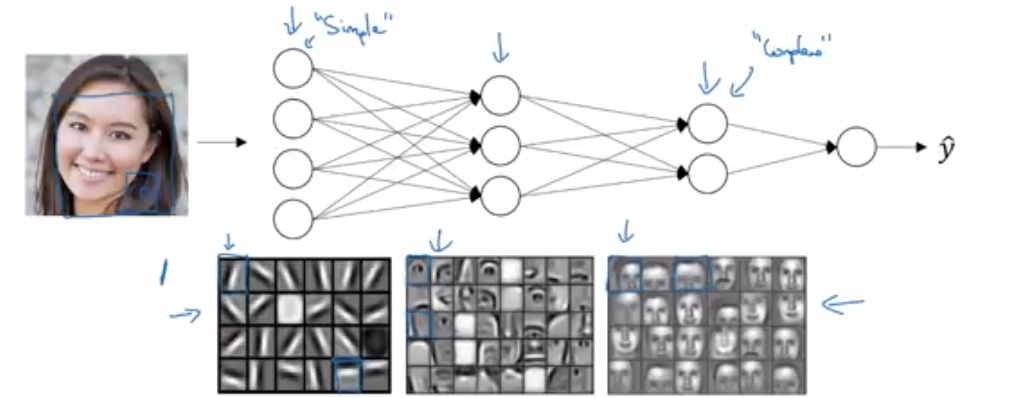
\includegraphics{./Images/c4week1/14-2.png}

\begin{itemize}
\tightlist
\item
  \textbf{합성곱 연산의 방식}\\
\item
  합성곱 연산은 합성곱 신경망의 핵심 요소
\item
  필터(또는 커널) 행렬을 입력 이미지의 왼쪽위에서부터 시작하여\\
  오른쪽과 밑으로 옮겨가며 대응 행렬 값끼리 곱한 후 모두 더해주는 방식.
\end{itemize}

 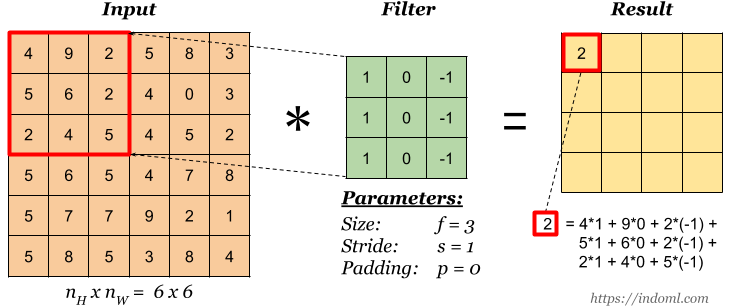
\includegraphics{./Images/c4week1/2-1.png} \\
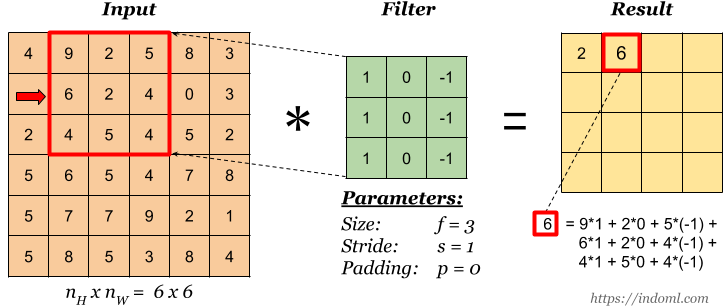
\includegraphics{./Images/c4week1/2-1-2.png}
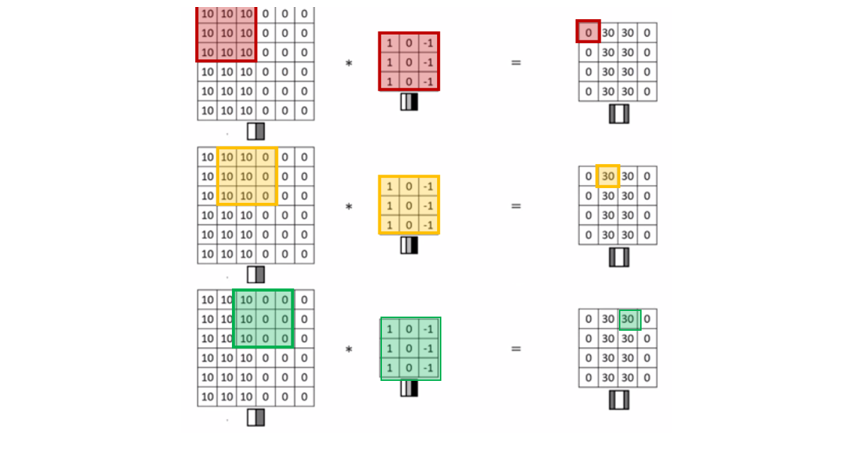
\includegraphics{./Images/c4week1/2-5.png} 

    \subsection{4.1.3. More Edge Detection}\label{more-edge-detection}

\begin{itemize}
\tightlist
\item
  \textbf{밝기 전환}\\
  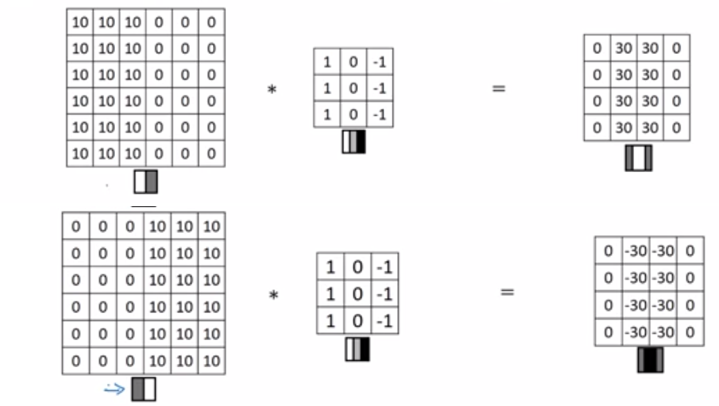
\includegraphics{./Images/c4week1/3.png} 
\end{itemize}

입력 이미지가 6 X 6 pixel의 Grayscale 이미지라면,\\
별도의 RGB 채널이 없기 때문에 6 x 6 x 3 의 행렬이 아닌 6 x 6 x 1 의
행렬이 된다.\\
위 사례에서 음영이 반대인 이미지를 뒤집어서 동일한 필터로 합성곱을 하여
결과 이미지에서 30 대신 -30 의 값이 얻어졌다.\\
그 결과 이미지의 가운데 구분 영역으로 입력 이미지의 가운데에 강한
경계선이 있을 뿐만아니라,\\
양과 음의 윤곽선의 차이로 인한 밝기의 전환을 확인할 수 있다. 두 종류의
차이가 중요하지 않다면, 결과 행렬에 절대값을 씌워줄 수 있다. -
\textbf{합성곱 필터의 종류} 
\includegraphics{./Images/c4week1/4-1-1.png}

\includegraphics{./Images/c4week1/4-0-2.png} CNN에서는 합성곱 필터
행렬의 값들이 parameter가 된다.\\
필터 행렬의 숫자 요소들을 변수로 두고 데이터로부터 학습함으로써
신경망이\\
이미지 내에서 윤곽선같은 하위 단계의 속성을 학습할 수 있게 된다.\\
 - \textbf{딥러닝 프레임워크의 합성곱 연산 함수} - Tensorflow:
tf.nn.conv2d - Keras: Conv2d

 

    \subsection{4.1.4. Padding}\label{padding}

\begin{itemize}
\tightlist
\item
  \textbf{합성곱 연산에서 이미지 축소의 문제점}

  \begin{itemize}
  \tightlist
  \item
    수백 개의 층을 거쳐 아주 작은 이미지만 남게 될 수 있다.
  \item
    이미지 가장자리의 정보들을 버리게 된다.\\
    \\
  \end{itemize}
\item
  \textbf{Padding} 이미지 축소의 문제점을 해결하기 위해 이미지를 덧대어
  입력값으로 넣어주는 변형 방식. 6 x 6 이미지의 가장자리에 1 픽셀만큼
  가장자리에 더해주면,\\
  기존의 8 x 8 이미지가 되어 3 x 3 필터와 합성곱을 한 후 동일한 6x6
  사이즈의 결과 이미지가 나온다.
  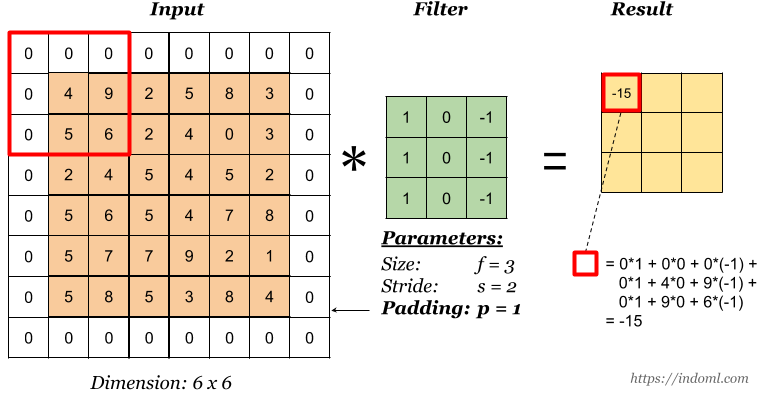
\includegraphics{./Images/c4week1/6-0.png} 
\end{itemize}

위 예시에서는 stride가 2라서 결과 이미지의 크기가 줄어들었지만,\\
stride가 0이라면 기존 이미지와 같은 6 x 6 크기를 얻게 된다.\\
따라서, padding을 하면 가장자리의 정보를 모두 취할 순 없지만 버리는 양을
줄일 수 있다.

\begin{itemize}
\tightlist
\item
  \textbf{패딩의 양 선택}
\item
  \textbf{Vaild (유효 합성곱)}: 패딩이 없는 경우.\\
  n x n 이미지, f x f 필터일 경우, 결과 이미지 (n - f + 1) x (n - f + 1)
\item
  \textbf{Same (동일 합성곱)}: 패딩이 있는 경우. 입출력 이미지 크기가
  동일.\\
  n x n 이미지, f x f 필터, p=패딩의 양일 경우, 결과 이미지 크기 = (n +
  2p - f + 1) x (n + 2p - f + 1)\\
  n = (n + 2p - f + 1)\\
  p = (f - 1) / 2

  \begin{itemize}
  \tightlist
  \item
    일반적으로 필터 크기 f x f 에서 f 는 3, 5, 7과 같은 홀수이다.\\
    f가 짝수이면 패딩이 비대칭이 되고,\\
    홀수의 경우에는 중심 위치가 존재하기 때문에 필터의 위치 파악이
    용이하다.
  \end{itemize}
\end{itemize}

 

    \subsection{4.1.5. Strided Convolutions}\label{strided-convolutions}

\begin{itemize}
\item
  \textbf{Stride}\\
  합성곱 필터 적용시 stride 값의 간격을 두어 칸을 옮기며 연산하는 것.\\
  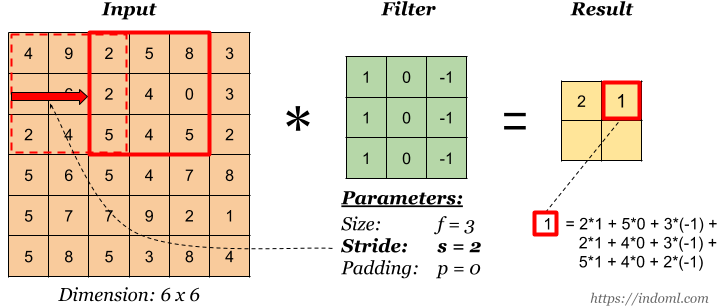
\includegraphics{./Images/c4week1/2-0.png} \\
   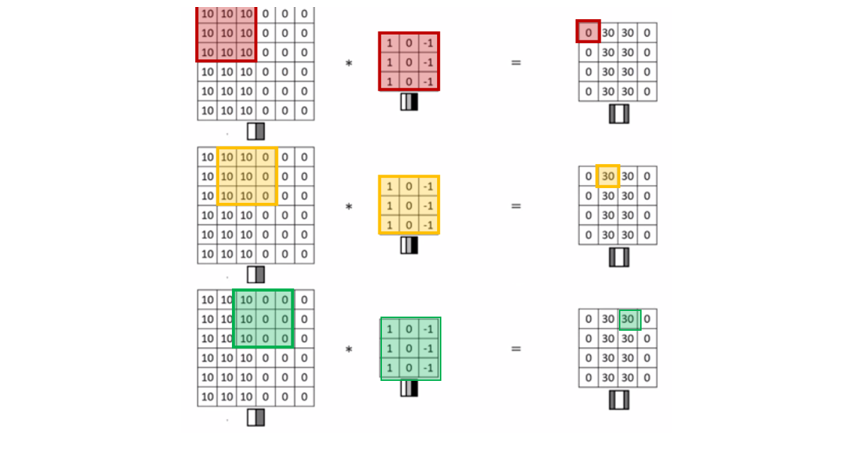
\includegraphics{./Images/c4week1/2-5.png}\\
\item
  \textbf{Strided Convolutions}\\
   
\includegraphics{./Images/c4week1/7-2.png}\\
   분수값이 정수가 아닐 경우 내림 연산하여 필터가 밖으로 나온 경우
  계산에 포함하지 않는다.\\
  일반적으로는 필터가 패딩된 이미지에 맞도록 설정한다. 
\item
  \textbf{Cross correlation과 Convolution}\\
  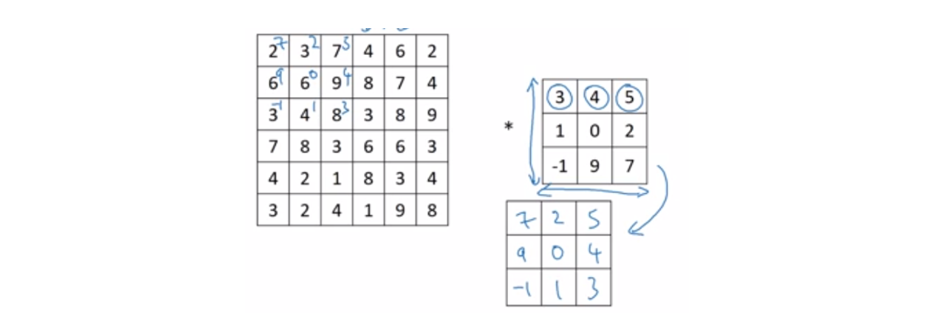
\includegraphics{./Images/c4week1/9.png}
\end{itemize}

일반적인 수학 교재에서 정의하는 Convolution은 가로축과 세로축으로 뒤집어
주는 mirroring 단계가 있다.\\
딥러닝 분야에서는 유용하지 않으므로 미러링 과정을 생략하므로\\
Cross correlation라고 해야 하지만, 관습적으로 Convolution이라 부른다. 

    \subsection{4.1.6. Convolutions Over
Volume}\label{convolutions-over-volume}

\begin{itemize}
\item
  \textbf{RGB 이미지 3D 필터}

  \begin{itemize}
  \tightlist
  \item
    너비x 높이x 채널의 수
  \item
    이미지의 채널 수와 필터의 채널 수가 일치\\
    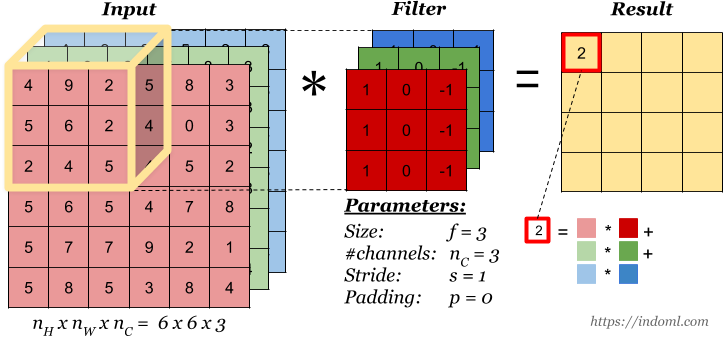
\includegraphics{./Images/c4week1/10-2.png} 
  \end{itemize}
\item
  \textbf{RGB 필터}
\item
  빨간색의 윤곽선을 감지하는 필터\\
  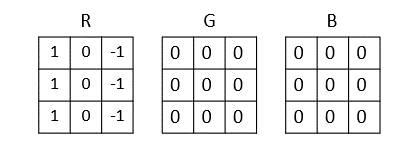
\includegraphics{./Images/c4week1/12.png}\\
\item
  특정색과 상관 없이 감지하는 필터\\
  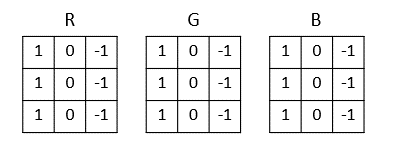
\includegraphics{./Images/c4week1/12-2.png}\\
\item
  \textbf{다중 필터}

  \begin{itemize}
  \tightlist
  \item
    세로와 가로, 또는 45도 혹은 70도 기울어진 윤곽선을 모두 감지\\
  \item
    검출하고자 하는 특성의 수 = 필터의 채널 수\\
     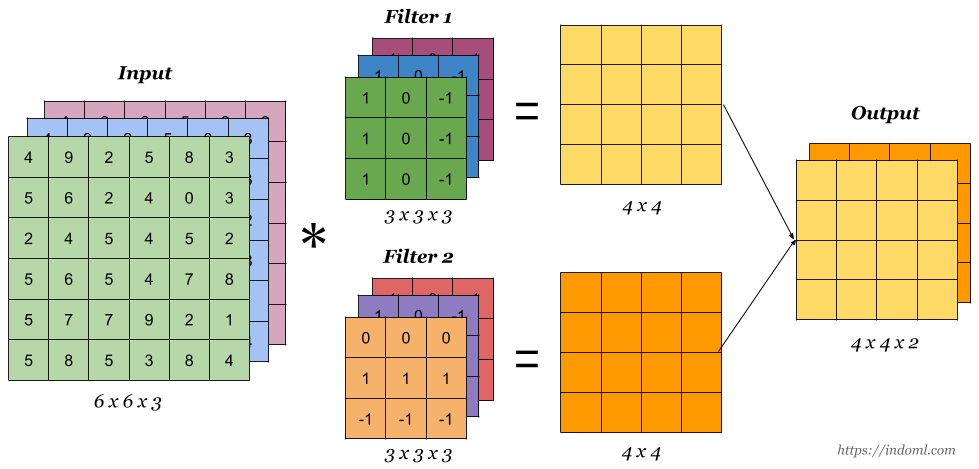
\includegraphics{./Images/c4week1/14-4.png}
  \end{itemize}
\end{itemize}

    \subsection{4.1.7. One Layer of a Convolutional
Network}\label{one-layer-of-a-convolutional-network}

\begin{itemize}
\item
  \textbf{Forward Propagation}\\
  
\includegraphics{./Images/c4week1/14-5-2.png}\\
\item
  \textbf{One Convolutional Layer}\\
   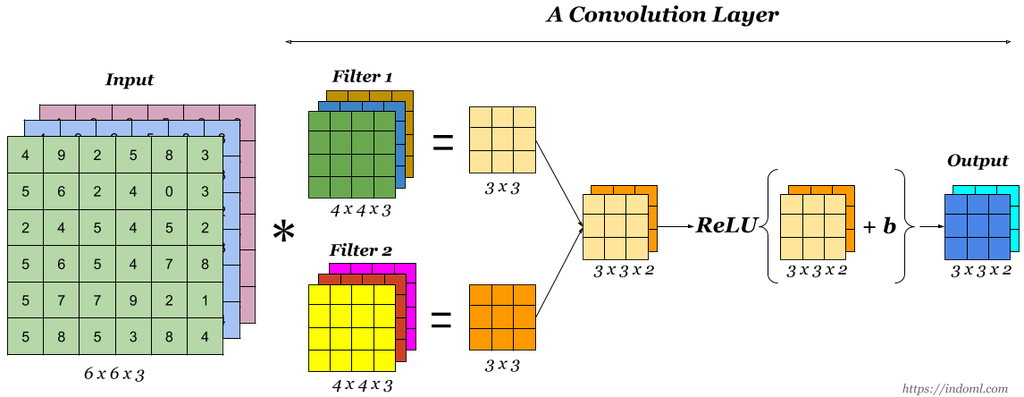
\includegraphics{./Images/c4week1/14-6.png}\\
   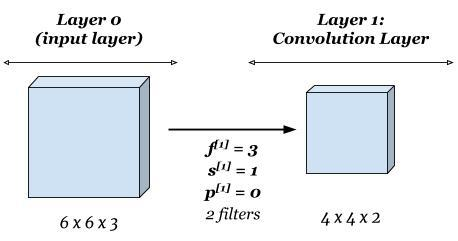
\includegraphics{./Images/c4week1/15.png}
  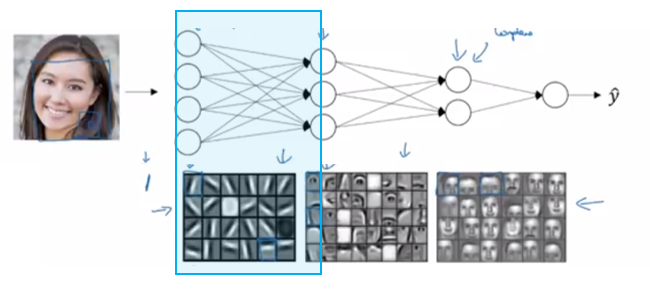
\includegraphics{./Images/c4week1/15-2.png} 
\item
  \textbf{Notation}\\
  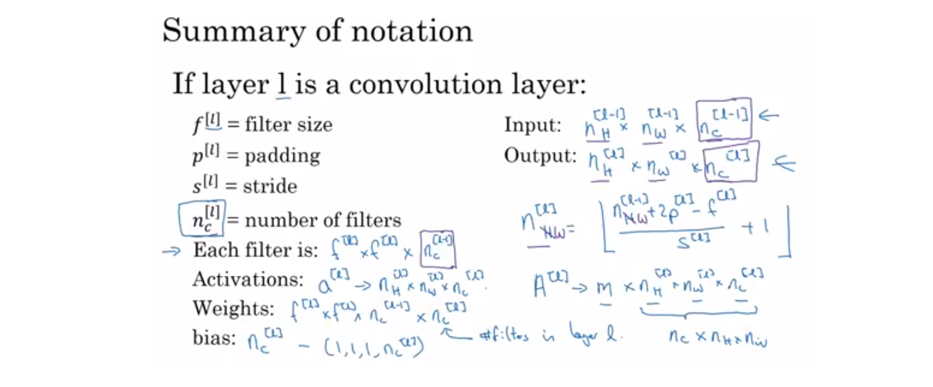
\includegraphics{./Images/c4week1/15-4.png} 
\end{itemize}

    \subsection{4.1.8. Simple Convolutional Network
Example}\label{simple-convolutional-network-example}

\begin{itemize}
\tightlist
\item
  \textbf{CovnNet Example}\\
\item
  신경망 깊이가 깊어질 수록 입력값의 높이와 너비가 줄어들고, 채널의 수는
  늘어나는 경향 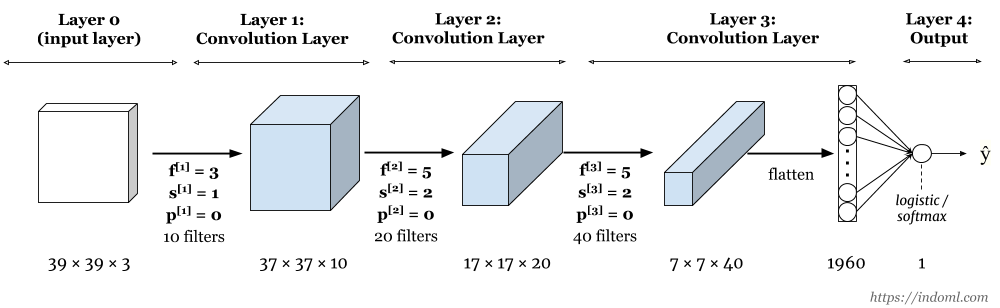
\includegraphics{./Images/c4week1/16.png} 
\item
  \textbf{Types of layer in CNN}\\
  -Convolution (CONV)\\
  -Pooling (POOL)\\
  -Fully Connected (FL)
\end{itemize}

     \#\# 4.1.9. Pooling Layers - \textbf{Pooling Layers}\\
표현 크기를 줄임으로써 계산 속도와 특성 검출의 정확도 증가\\
 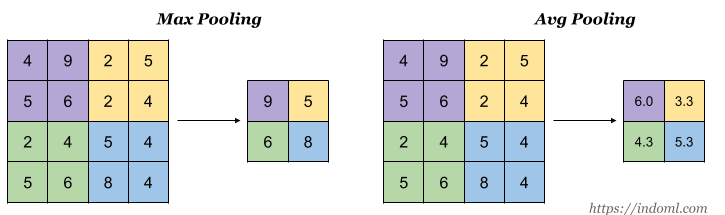
\includegraphics{./Images/c4week1/17.png} \\
 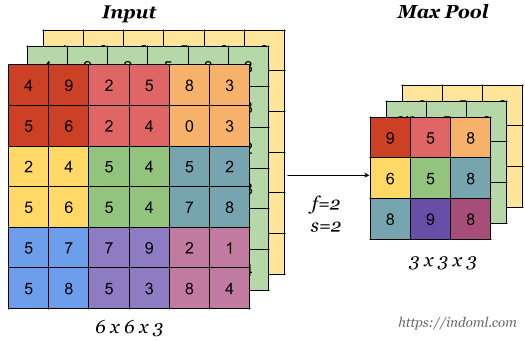
\includegraphics{./Images/c4week1/17-2.png}

\begin{itemize}
\tightlist
\item
  \textbf{hyper-parameters}

  \begin{itemize}
  \tightlist
  \item
    filter size (\emph{f})
  \item
    stride (\emph{s})
  \item
    pooling type (max or avg)
  \end{itemize}
\item
  hyper-parameter가 고정값이기 때문에 gradient descent로 학습 하지
  않는다.
\item
  f = 2, s = 2: 높이와 너비를 절반으로 줄임
\end{itemize}

    \\
\#\# 4.1.10. CNN Example 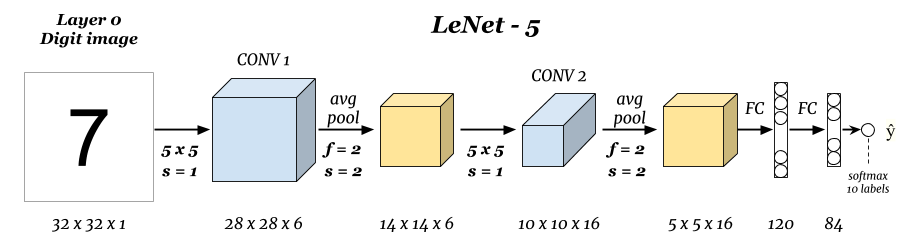
\includegraphics{./Images/c4week1/18.png}\\
 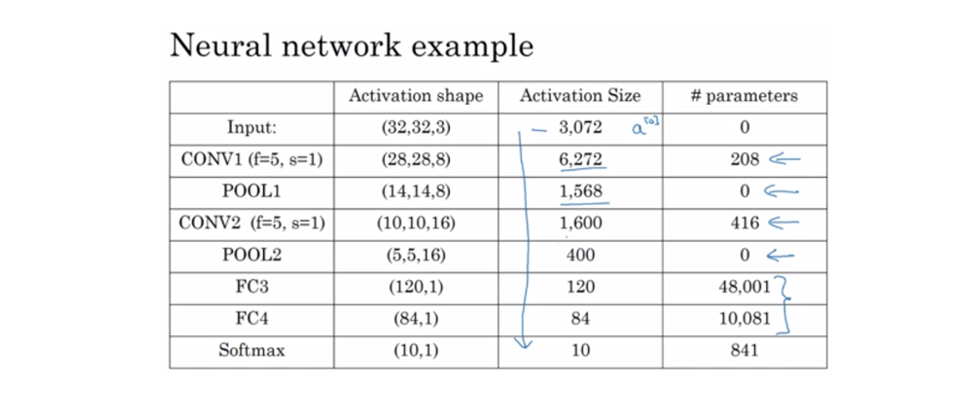
\includegraphics{./Images/c4week1/18-3.png}\\
 - \textbf{신경망의 층의 개수}: 일반적으로는 가중치와 변수를 가지는 층을
말한다.\\
Pooling layer는 가중치와 변수가 없고 하이퍼파라미터만 있기 때문에,
CONV와 POOL을 하나의 층(Layer) 으로 묵는다.

     \#\#\# 4.1.11. Why Convolutions? - \textbf{Convoltion의 장점} -
\textbf{Parameter sharing}: 입력 이미지의 여러 위치에서 동일한 필터를
사용함으로써 학습해야 할 parameter의 갯수 감소. - \textbf{Sparsity of
Connection}: 입출력 결과가 필터의 크기만큼만 영향을 받아 parameter의
갯수 감소

    \paragraph{Additional Reference}\label{additional-reference}

https://indoml.com/2018/03/07/student-notes-convolutional-neural-networks-cnn-introduction/


    % Add a bibliography block to the postdoc
    
    
    
    \end{document}
